\subsection{Architectuur}
\label{subsec:architectuur}

De architectuur van een applicatie die Canvas.hs gebruikt bestaat uit drie componenten. De applicatie van de gebruiker, de Canvas.hs module en de JavaScript Canvas.hs applicatie. De Canvas.hs module biedt functies aan die de programmeur kan gebruiken om te tekenen en bepaalde acties uit te voeren in de browser. De module draait een server om te communiceren met de browseromgeving. De browseromgeving verbindt door middel van websockets met de server en geeft de output van het programma weer in een canvas HTML-element. In \autoref{fig:architectuur} is een schematische weergave van de architectuur weergegeven.

\begin{figure}
\begin{center}
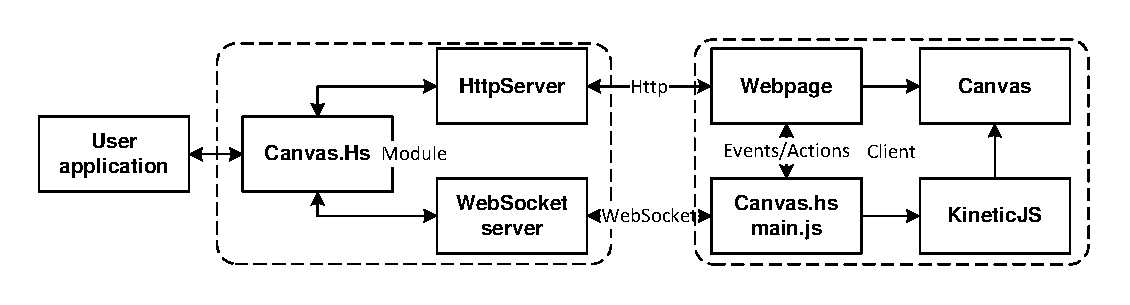
\includegraphics[keepaspectratio,width=\textwidth]{./images/architecture.pdf}
\caption{Architectuur van Canvas.hs}
\label{fig:architectuur}
\end{center}
\end{figure}

\subsubsection{Communicatie}
Gegevensoverdracht tussen de HTTP server en de browser moet snel gebeuren. Om de grafische elementen in de browser weer te geven moeten de output van de grafische interface naar de browser gecommuniceerd worden. Wanneer de gebruiker interactie heeft met de interface moet dit naar het programma van de gebruiker gecommuniceerd worden. Verder zal het programma bepaalde acties moeten kunnen uitvoeren op de webbrowser, zoals fullscreen laten gaan van de browser. Een belangrijke overwegingen is dat de grafische interface zo min mogelijk vertraging moet hebben.


\paragraph{Websockets}
Het is mogelijk om door middel van XMLHttpRequest of WebSockets een verbinding te onderhouden tussen de Module en de Clientomgeving. XMLHttpRequests worden door alle webbrowsers ondersteund, en kan door middel van longpolling technieken (Comet) een verbinding onderhouden met de webserver. De meest recente browsers ondersteunen WebSockets. Dit biedt een socket verbinding tussen de client en de server. Het WebSockets protocol biedt een betere performance dan alle technieken op basis van XMLHttpRequests en biedt een groter implementatiegemak. Door het gebruik van het HTML canvas element zal de browser ondersteuning al beperkt zijn tot de meest recente browsers. Canvas.hs maakt gebruik van WebSockets.

\paragraph{Protocol}
Het formaat van het protocol is JSON\todo{JSON moet nog toegelicht worden}, dit is praktisch doordat dit eenvoudig in JavaScript te gebruiken is. In tegenstelling to XML heeft JSON bovendien weinig overhead.

Het protocol tussen de client en de server bevat voornamelijk interface data. De structuur en de attributen moeten vertaald worden van de Haskell omgeving om gebruikt te worden om te tekenen in het Canvas en vervolgens input van de gebruiker in de browseromgeving te ondersteunen. Voor optimale performance wordt de structuur zo snel mogelijk vertaald naar de structuur van KineticJS\todo{Kinetic moet ge\"introduceerd worden en toegelicht worden}. De programmeur bepaalt wanneer er interface data verstuurd word en wanneer acties verstuurd worden naar de client.

\paragraph{Stateless client}
In functioneel programmeren is het gebruikelijk\todo{gebruikelijk, veel gebruik te maken? dat is een beetje een vage aannamen} om veel gebruik te maken van functies die puur werken zonder state bij te houden in verschillende variabelen. In de huidige opzet van het vak functioneel programmeren biedt de grafische module een state object aan waarin de gebruiker alle state variabelen in kan opslaan. Wanneer de gebruiker de grafische interface updatet doet hij dit door de volledige boom van grafische elementen aan te passen of over de huidige output te tekenen. Dit maakt het overzichtelijk voor de programmeur omdat de grafische interface dan geen eigen state bijhoudt. Dit maakt de grafische interface op de client stateless. Een groot nadeel hiervan is dat iedere keer dat de grafische interface geupdated wordt ook de volledige grafische output weer naar de client verstuurd dient te worden. De enige state die de client vasthoudt wordt veroorzaakt door acties.

Een alternatief voor het versturen van volledige grafen is een vorm van delta updates, waarbij de programmeur opgeeft wat er veranderd is in de inteface of dat de module zelf uitvindt welke delen in de boom aangepast zijn. Beide mogelijkheden voegen veel extra complexiteit toe, voor respectievelijk de programmeur en voor het systeem. De bandbreedte van lokale websockets is groot en heeft geen last van latency waardoor de performance van de connectie hierdoor niet beperkt wordt.
